\documentclass[10pt,conference,compsocconf]{IEEEtran}

\usepackage{hyperref}
\usepackage{graphicx}	% For figure environment
\usepackage{authblk}
\usepackage{tabularx}
\usepackage{algorithm}
\usepackage{algorithmic}
\usepackage{float}

\title{Project 2 on Machine Learning\\Text classification\\Team Yoor}

\author[1]{Sergei Volodin}
\author[1]{Omar Mehio}
\author[1]{Baran Nama}
\affil[1]{EPFL}
\affil[ ]{\textit {\{sergei.volodin,omar.mehio,baran.nama\}@epfl.ch}}

\begin{document}

\maketitle

\begin{abstract}
A classification dataset consisting of Tweets is being studied. First, the data is thoroughly explored using visual aids. Several basic Natural Language Processing methods are applied. Results are evaluated using cross-validation. Model overview is given and the best model is chosen.
\end{abstract}

\section{Introduction}
This paper investigates into improving the quality of sentiment analysis on Tweets dataset \cite{kaggle}.
It consists of $N_1=N_2=1250000$ positive/negative tweets, each of them representing a message in English and numerical alphabet $\Sigma$ with no longer than 140 characters.
This way, each of $N=N_1+N_2=2500000$ tweets is assigned to one of the classes $\mathcal{C}=\{\mbox{:(},\,\mbox{:)}\}$.
The task is to minimize the classification error.
In other words, if $\mathcal{D}=\{(x_n, y_n)\}_{n=1}^N$ is the dataset with tweets $x_i\in\Sigma^*$ being messages and $y_n\in \mathcal{C}$ being class labels, the goal is to train a classifier $f\colon\, \Sigma^*\to\mathcal{C}$ which minimizes the loss function $l(y,\hat{y})=[y\neq \hat{y}]$.

The task of sentiment analysis of tweets was thoroughly studied \cite{sota1, sota2, sota3, sota4}. These solutions usually give accuracy around 80\%.
Several techniques were applied, mostly consisting of two steps.
First, the words are converted to dense vectors using Glove, word2vec, cbow or skip-gram models.
After that, the resulting word vectors are used to construct features for the whole tweet.
At the end, the vector is feeded into a classifier, such as SVM or Logistic Regression.
Two latter steps might be replaced with a neural network accepting variable-length input such as CNN.
Moreover, the embeddings themselves might be trained using backpropagation while training the classifier.

Claim: it is possible to find a model which fits the data better than the current state-of-the-art using expert knowledge on the Tweets dataset.

Next sections describe in details our approaches and compare them to various baselines.
\section{Models and Methods}
\subsection{Data cleaning}
\newcolumntype{L}[1]{>{\hsize=#1\hsize\raggedright\arraybackslash}X}%
\newcolumntype{R}[1]{>{\hsize=#1\hsize\raggedleft\arraybackslash}X}%
\newcolumntype{C}[1]{>{\hsize=#1\hsize\centering\arraybackslash}X}%

\begin{table*}[htbp]
	\centering
	\small
	\begin{tabularx}{\textwidth}{| L{0.1} | L{0.05} | L{0.7} | L{0.2} | }
		\hline
		Class&Row&Message&Comment\\
		\hline
		:( & 171 & {\tt <user> 5k i could cry i'm so unfit !} & User tag \\\hline
		:( & 99804 & {\tt if i feel like this tomorrow i'm going to the er } & Contraction, missed comma\\\hline
		:) & 524 & {\tt its the weekend ! ! <user> s coming home anddd <user> s baby shower , exciteddd } & Letter repetitions\\\hline
		:) & 99615 & {\tt <user> aren't you just an adorable granny <url> } & URL tag\\\hline
		:) & 443 & {\tt <user> :d :d :d :d :d wish jocelyn had a twitter . \#kudos for her too . } & Hashtag, emoticons \\\hline
		:) & 468 & {\tt retweet if you was born in the 90 ' s ! \#90's babies } & Grammar\\\hline
		:( & 14 & {\tt <user> i'm white . \#aw } & Appear neutral \\\hline
		:( & 99594 & {\tt <user> <user> <user> they're there tonight ! ! ! } & Appear positive \\\hline
	\end{tabularx}
	\caption{Examples of tweets in the small dataset}
	\label{tab:tweet-sexample}
\end{table*}

This paragraph describes the data being studied.
Tweets are short messages no longer than 140 characters long \cite{twitter}.
The table \ref{tab:tweet-sexample} represents a few examples from the small dataset.
Being considered an informal way of communication, tweets often contain misspelled words and letter repetitions, grammatical and other writing mistakes.
Besides plain text with punctuation, tweets also contain hashtags, two types of tags, {\em user} and {\em url}, which are tokens for replaced user mentions and URL links, respectively.
In addition, tweets sometimes contain emoticons.
Despite the fact that objects in the training dataset mostly comply with its classes, some tweets cannot be determined as positive/negative even by a human (appear neutral).
Moreover, some of the tweets are clearly mislabeled in the training data.
Dataset contains repeating tweets.

\begin{figure}[!htb]
	\centering 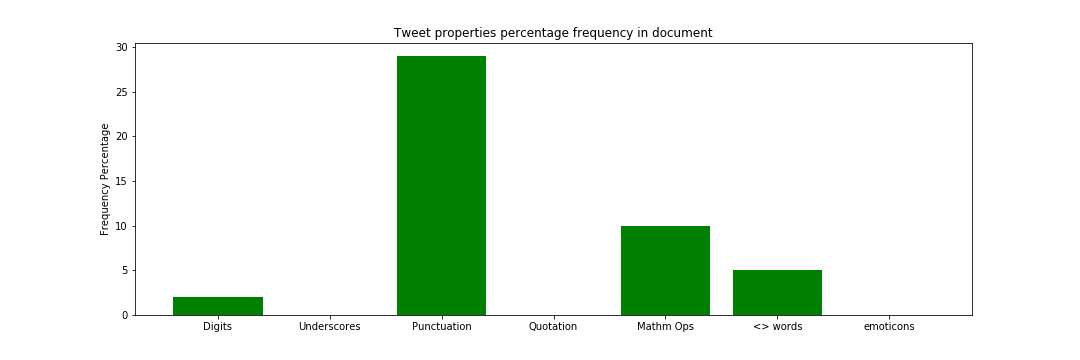
\includegraphics[width=0.5\textwidth]{../plots/types.png}
	\caption{Distribution of Tweet properties}
	\label{prop}
\end{figure}

The first step taken was exploring special properties of tweets in the datasets. These properties include hashtags, punctuation and are present in huge percentages (Fig \ref{prop}). Through preprocessing the aim was to maximize the knowledge that can be extracted from the datasets in order to build word representations, which is achieved through correction of misspelled words and stemming techniques.

Usually tweeters repeat a letter in a word to stress on a certain emotion, as an example: "i am soooooo angryyyy". This problem was tackled by two different approaches. The first approach is stemming, which is defined as the process by which every word is replaced by it's origin. Linguistically any word can be changed to different forms by either adding affixes or prefixes. Through stemming, the aim is to minimize the presence of these different forms and replacing them with the original stem. The stemming algorithm presented in \ref{Stemming} solves the mentioned problem.

\begin{algorithm}
\caption{Stemming(token)}
\label{Stemming}
\begin{algorithmic} 
\IF{token in dictionary}
\STATE return token
\ELSE
\STATE $X \leftarrow $ token with repeating character replaced by two instances of that character
\IF  {X == token}
\STATE return token
\ELSE
\STATE return Stemming(X)
\ENDIF
\ENDIF
\end{algorithmic}
\end{algorithm}


The second approach adopted is misspelling correction. The process goes as follows: a token in the tweet is proposed to an English dictionary, the dictionary responds by either indicating that the word is valid or not. This dictionary provides the most relevant suggestions to correct a wrong token. The levenshtein distance was used to determine whether a word should be converted to the suggestion or not. Levenshtein distance is defined as: "the distance between two strings is the minimal number of insertions, deletions, and substitutions of one character for another that will transform one string into the other". Thus to explore how many misspelled words are in the dataset, we plotted the distribution in Fig. \ref{levDistA}. Most of the data can be covered by setting our levensteihn threshold to 4.
\begin{figure}[!htb]
	\centering 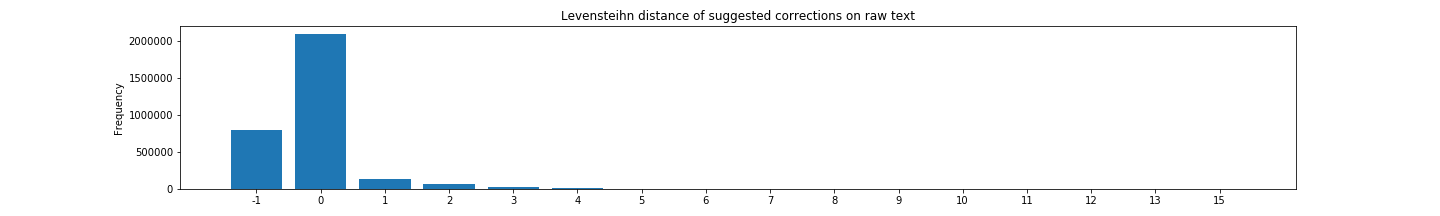
\includegraphics[width = 0.5\textwidth]{../plots/distributionA.png}
	\caption{Levensteihn distance distribution on raw tweets}
	\label{levDistA}
\end{figure}

\begin{figure}[!htb]
	\centering 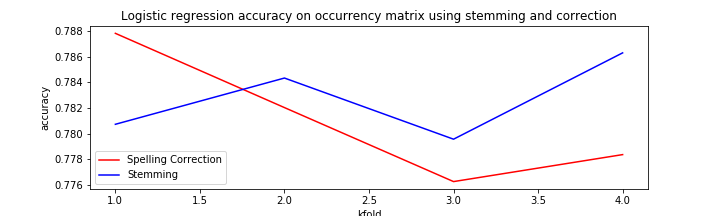
\includegraphics[width=220px]{../plots/raw.png}
	\centering 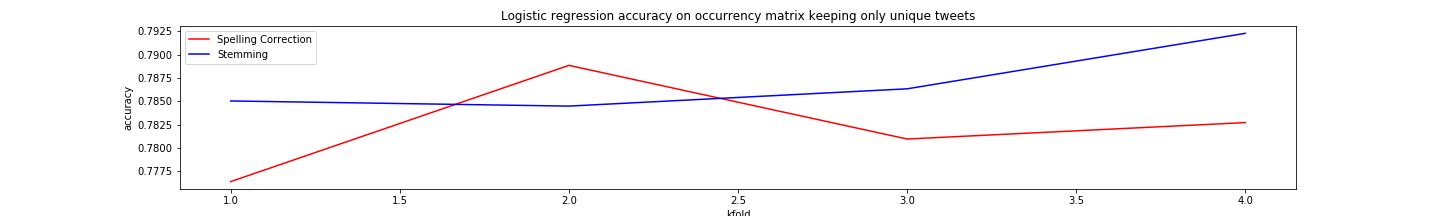
\includegraphics[width=220px]{../plots/redundant.png}
	\caption{Logistic Regression accuracy on correct and stemmed tweets}
	\label{raw}
\end{figure}

The metric used to compare both methods was prediction accuracy of logistic regression. As a first step the combined dataset of both the positive and negative tweets was exposed to stemming and correction. Then for each method a vocabulary of words is constructed. Finally, the occurrence matrix is built from both the tweets and the dictionary. K-fold is used to split the matrix and then logistic regression is run using the occurrence matrix as the data matrix, labels are split into 0 denoting positive sentiment and 1 denoting a negative sentiment.  As observed in Fig. \ref{raw}, the spelling correction method is superficial to the stemming method with reaching a maximum of 78.8 \% prediction accuracy.


Another property of the dataset is the presence of redundant tweets. To view their impact, repeated instances of a tweet are eliminated and the newly formed unique dataset is exposed to the previous methods. The stemming technique overpowers the misspelling correction technique. Although with very small improvement in accuracy prediction (79\%).

\begin{figure}[!htb]
	\centering 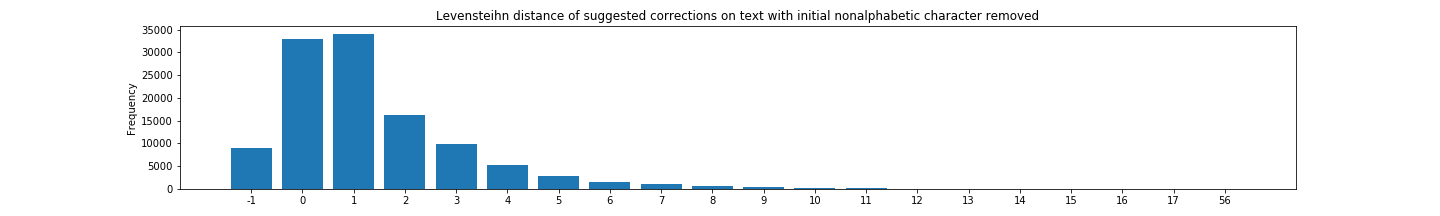
\includegraphics[width=0.5\textwidth]{../plots/distributionB.png}
	\caption{Levensteihn distance distribution on tweets with non-alphabetic starting character stripped}
	\label{levDistB}
\end{figure}

Tokens in our datasets starting with non alphabetic characters were eliminated from previous experiments as all dictionaries can't recognize non alphanumeric words. Thus a new set of tweets was constructed having all these tokens stripped of the initial non-alphabetic character or characters. As before, the distribution of levensteihn distances (Fig. \ref{levDistB}) for suggested words was plotted, which results in a more uniform distribution.

\begin{figure}[!htb]
	\centering 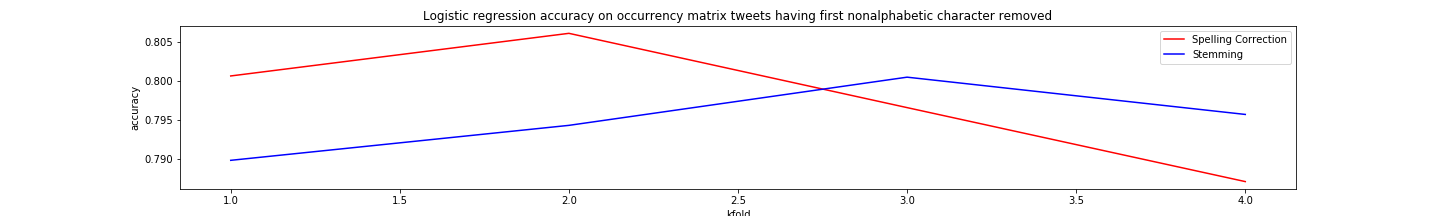
\includegraphics[width=0.5\textwidth]{../plots/filtered_text.png}
	\caption{Logistic Regression accuracy on tweets with non-alphabetic starting character stripped }
	\label{filtered}
\end{figure}

The newly constructed dataset is subject to previous methods. Elimination of redundant tweets,stemming and misspelling correction. Accuracy prediction then improves to 80.2\%, the best score reached so far.

\begin{figure}[!htb]
	\centering 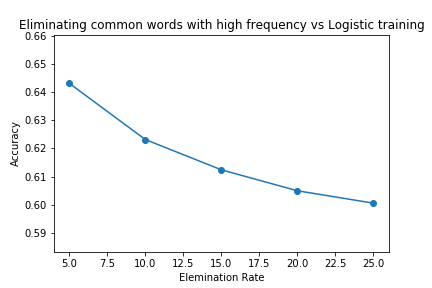
\includegraphics[width=100px]{../plots/commonElem.png}
	\centering 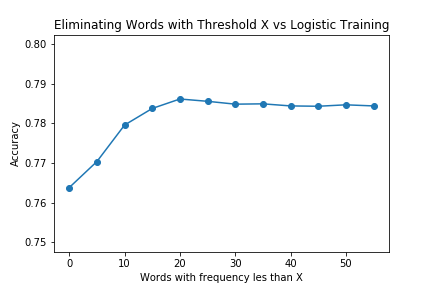
\includegraphics[width=100px]{../plots/nonfrequent.png}
	\caption{Elimination of common frequent terms vs separate non-frequent terms}
	\label{freq}
\end{figure}
Now with the optimal model having initial non-alphabetic characters removed, redundant tweets eliminated and misspelling correction applied with levensteihn threshold set to 5. The dataset is tackled from a different angle, the effect of the frequency of which one token appears in the document is explored. Thus two approaches are considered: removing most frequent tokens that are common in both datasets and removing non-frequent words from the combined vocabulary set. The results of the first experiment came as a surprise, since we suspected that elimination of common words would make it easier for the classifier to distinguish between a positive sentiment tweet and a negative one. A reasoning contributed for such results is the limited number of characters provided for users to express themselves and thus most of the tweet content gets distributed among tagging other users, using punctuation and stop words. The second approach was of more relevance, where elimination of non frequent tokens from the vocabulary has helped improving accuracy to 78\%, as observed in Fig. \ref{freq}.

\subsection{Prediction models}
\subsubsection{GloVe embeddings}
Several models were considered.
First, the baseline was the GloVe \cite{glove} model, which considers training embeddings on the co-occurence matrix. The pre-trained embeddings (Twitter, Stanford NLP group) with dimensions of 100 and 50 were used. Higher dimension embeddings did not fit to the server memory.

\subsubsection{Word count model}
Secondly, a word count model was considered as a baseline solution because of its simplicity. This model uses high. A tweet is represented by a high-dimension sparse vector, each item corresponds to a number of occurrences of a word in the tweet.
This vector was further classified using several techniques, such as SVM and Neural Network.
This method gave accuracy which placed the team to the 47/66 place in the public Kaggle leaderboard and allowed for tweaking its parameters with relatively small training time (a Google Cloud instance with 8 CPU was used).
This model was trained both on raw and preprocessed data. Raw data gave higher score, when using preprocessed data resulted in overfitting. A reduction of the vocabulary size was also considered by taking only words occurring most frequently.
\subsubsection{Convolutional neural networks (CNN)}

Representation of tweets were in a 1d vectors, where convolutional layers are summed in sequential manner. Due to small size of the embeddings, pooling layers were not used between convolutional layers. Dropout layers were performed before output layer and between convolutional layers \cite{cnn5} in order to prevent overfitting. For hidden layers, ReLU is used, for first two elements of output layer tanh activation function is used and for the last element of output layer, softmax activation function is used in favor of common practice \cite{cnn6}.
Note that, the number of filters for convolutional layers, the size of the filters, activation function types regarding the type of the layer, dropout amount and the number of convolutional layers are just a subset of complete hyper parameters of this model that were not regulated.

\section{Results}
\begin{table}[ht]
	\centering
	\small
	\begin{tabular}{|c | c |  c | c | c |} 
		\hline
		Model & Dataset & Train acc. & Val. acc. & L2 \\
		\hline
		GloVe FC & Full & 0.62 & 0.62 & $10^{-6}$\\
		\hline
		WC LR & Partial & 0.86 & 0.81 & 1000, not tuned\\
		\hline
		WC LR & Full & 0.86 & 0.83 & 1000, not tuned\\
		\hline
		WC FC 100x50 & Full & {\bf 0.87} & {\bf 0.86} & 1000, not tuned\\
		\hline
		WC FC 100x50 & Full, clean & 0.82 & 0.83 & 1\\ [1ex] 
		\hline
	\end{tabular}
	\caption{Comparison of different methods (WC=Word Count, GloVe~-- pretrained GloVe vectors, LR~-- Logistic Regression, FC~-- fully-connected, WC~-- word count)}
	\label{tab:results}
\end{table}

The following models were considered: CNN, Logistic Regression, Fully Connected Neural Network. Moreover, a simple word count model was considered. The best model was the word count model on raw data. However, proper hyperparameter tuning was not performed, this, it is not possible to claim that it is better than other models. Our contribution consists of cleaning tweets and proving that it's possible to classify them using a simple word count model.
\section{Discussion}
Despite performing data cleaning, we were not able to run all of the models on cleaned data. Moreover, the hyperparameter tuning was not performed in a proper way.
\section{Summary}
We have considered tweet classification task. Each tweet, consisting of no more than 140 alphanumeric characters, must be assigned to one of the classes: positive or negative sentiment. Data was cleaned by correcting spelling mistakes. Several models were considered: CNN, FC NN on pretrained GloVe embeddings, and simple word count model with FC NN. In this project, the word count model on raw data proved to be the most efficient. However, hyperparameters were not properly tuned for the models considered.

\begin{thebibliography}{99}

	\bibitem{twitter} \href{http://twitter.com}{Twitter}
	\bibitem{sota1} Go, Alec, Lei Huang, and Richa Bhayani. "Twitter sentiment analysis." Entropy 17 (2009): 252.
	\bibitem{sota2} Kouloumpis, Efthymios, Theresa Wilson, and Johanna D. Moore. "Twitter sentiment analysis: The good the bad and the omg!." Icwsm 11.538-541 (2011): 164.
	\bibitem{sota3} Tapan Sahni, Chinmay Chandak, Naveen Reddy, Manish Singh. "Efficient Twitter Sentiment Classification using Subjective Distant Supervision"
	\bibitem{sota4} Alec Go, Richa Bhayani,	Lei Huang. "Twitter Sentiment Classification using Distant Supervision"
	\bibitem{glove} Jeffrey Pennington, Richard Socher, Christopher D. Manning. "GloVe: Global Vectors for Word Representation"
	\bibitem{cnn5} Park, S., and Kwak, N. (2016, November). "Analysis on the Dropout Effect in Convolutional Neural Networks." In Asian Conference on Computer Vision (pp. 189-204). Springer, Cham.
	\bibitem{cnn6} http://cs231n.github.io/neural-networks-1/{\#}actfun
\end{thebibliography}
\end{document}
